\section{Simulation}

\subsection{DRO10000A Voltage Controlled Oscillator} \label{DROSimulation}
The Dielectric Resonator Oscillator was simulated by its mathematical output in MATLAB. Given that our DRO outputs 0 dBm at 10GHz, we can plot and visualize the carrier frequency. Since we are given the frequency, we can assume the sinusoidal aspect of the wave to be 
\begin{equation}
    carrierWave = cos(2\pi f_0 t), \ \ \ f_0 = 10GHz
\end{equation}

Following that, we must determine amplitude. We can use the simple power equation
\begin{equation}
    P = \frac{V\textsubscript{peak}^2}{2}
\end{equation}
We can also define the power of the signal to be
\begin{equation}
    P = 10^{\frac{P\textsubscript{dBm}}{20}}*cos(2\pi f_0 t)
\end{equation}

Putting it all together, we get the following equation representing the DRO:
\begin{equation}
    V\textsubscript{peak} = (\sqrt{2* 10^{\frac{P\textsubscript{dBm}}{20}}}) * cos(2\pi f_0 t)
\end{equation}

Thus, in MATLAB, we can use the following line:
\inputminted[breaklines]{Matlab}{./Code/DRO_Simulation.m}

\begin{figure}[H]
    \centering
    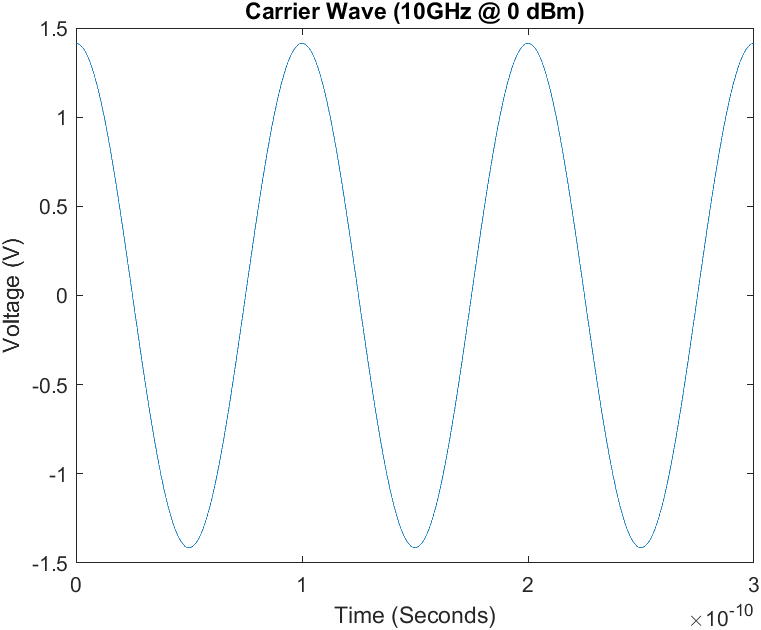
\includegraphics[width = 0.6\textwidth]{Images/CarriervTime.png}
    \caption{Simulation of a 10GHz signal at 0dBm}
    \label{fig:carrierVTime}
\end{figure}


\subsection{OPA207 Inverting Summing Amplifier}
Through nodal analysis, we have derived equation \eqref{invertingAmp}. Thus, simulating the inverting summing amplifier is as simple as plugging in our computed values.
\inputminted[breaklines]{Matlab}{./Code/OpAmp_Simulation.m}

\begin{figure}[H]
    \centering
    \begin{subfigure}[b]{0.48\textwidth}
        \centering
        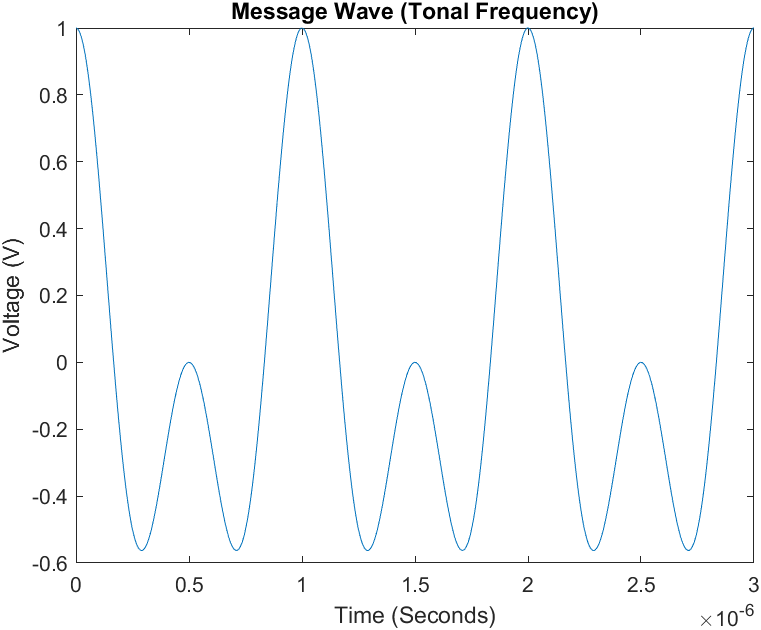
\includegraphics[width = 1\textwidth]{Images/MessagevTime.png}
        \caption{Original Message vs Time}
        \label{fig:messageVTime}
     \end{subfigure}
     \hfill
     \begin{subfigure}[b]{0.48\textwidth}
        \centering
        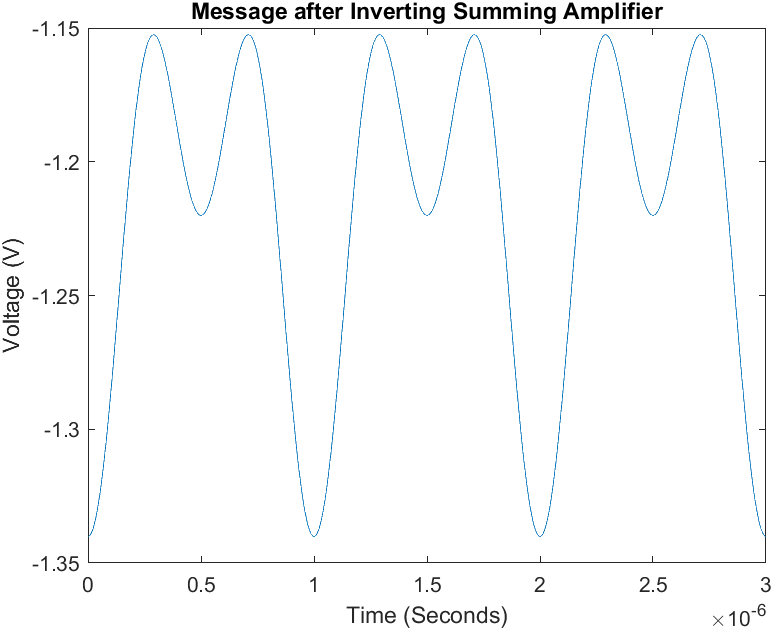
\includegraphics[width = 1\textwidth]{Images/AfterInverting.png}
        \caption{After the Inverting Summing OpAmp}
        \label{fig:opAmpVTime}
     \end{subfigure}
        \caption{Message Wave before and after the inverting summing op-amp}
        \label{fig:Both Graphs}
\end{figure}

\begin{figure}[H]
    \centering
    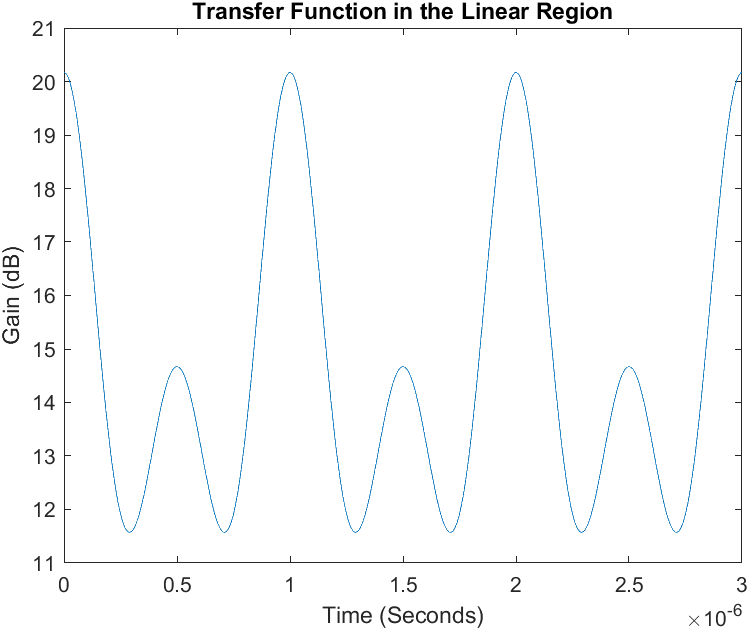
\includegraphics[width = 0.6\textwidth]{Images/Message Gain.png}
    \caption{Message Gain as a function of time}
    \label{fig:Gain}
\end{figure}

\subsection{HMC694LPE Variable Gain Amplifier}
    \paragraph{Linear Region Gain}
    As mentioned in \ref{VGA Linear}, we found that the linear region of the Variable Gain Amplifier would be the most useful. As Control Voltage varies, so too does the gain of the VGA, linearly. Thus, to simulate, we must determine the slope and the y-intercept. Instead of manually computing, we made the choice to recompute this regression everytime. If ever a more accurate regression was necessary, it would be as simple as slotting more datapoints into our model.
    
    \inputminted[breaklines]{Matlab}{./Code/VGASim.m}
    
    \begin{figure}[H]
        \centering
        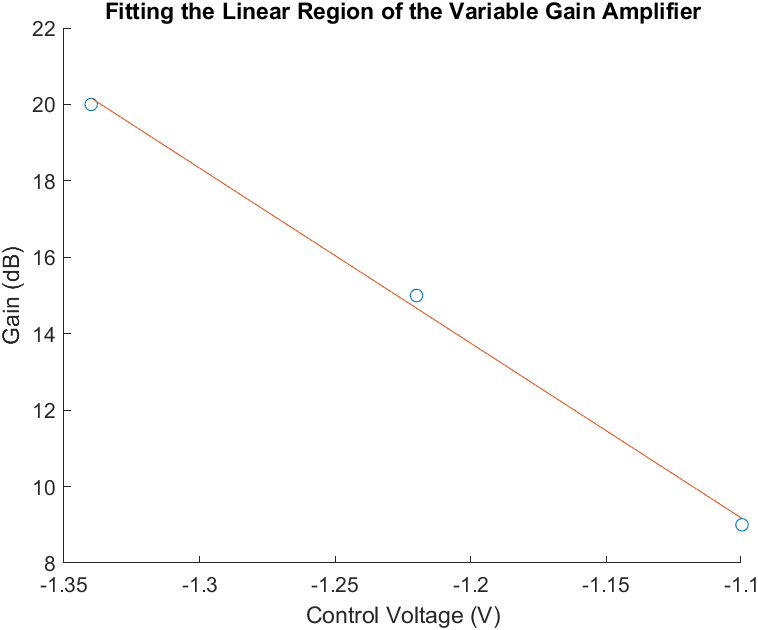
\includegraphics[width = 0.6\textwidth]{Images/LinearRegression.png}
        \caption{Regression plotted against the measured values}
        \label{fig:regression}
    \end{figure}

    \paragraph{Amplifier}
    
    Once obtaining the gain produced by the control voltage, we need to add it to our original carrier wave and convert back into voltage.
    \inputminted[breaklines]{Matlab}{./Code/VGASim2.m}
    

    \begin{figure}[H]
        \centering
        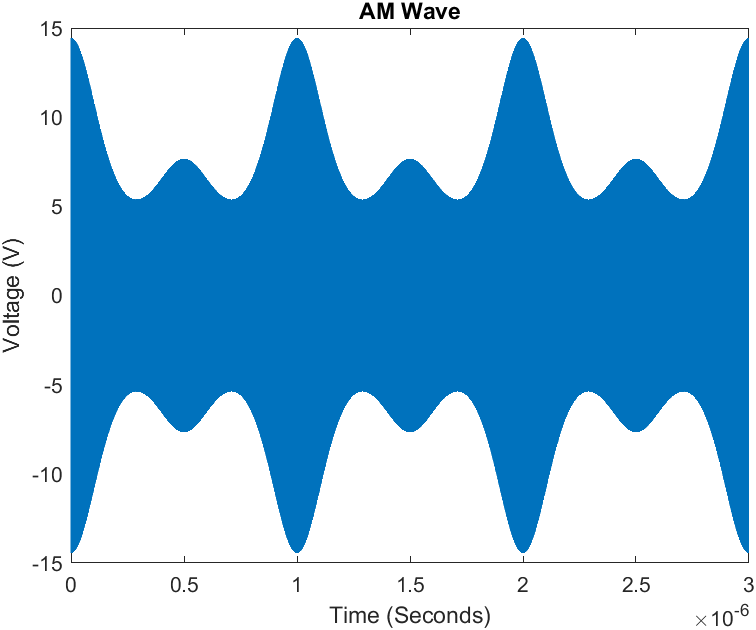
\includegraphics[width = 0.6\textwidth]{Images/AMWave.png}
        \caption{The Amplitude Modulated Wave}
        \label{fig:AM}
    \end{figure}

\newpage
\subsection{YAT-30A+}
    Though we now have an amplitude modulated wave, it doesn't conform to 15dBm. Thus running the signal through the 30dB attenuator nets the following waveform:
    \inputminted{Matlab}{./Code/FinalWave.m}
    \begin{figure}[H]
        \centering
        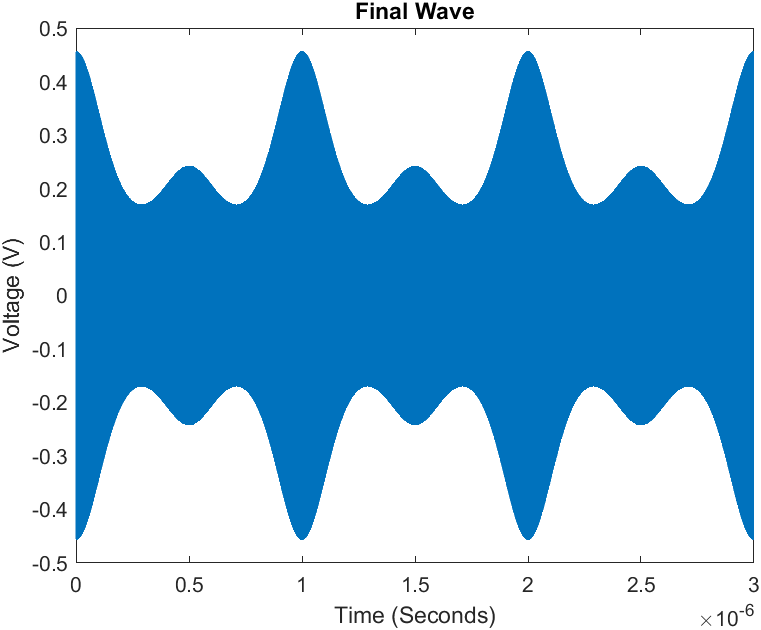
\includegraphics[width = 0.6\textwidth]{Images/FinalWave.png}
        \caption{The final attenuated Amplitude Modulated Wave}
        \label{fig:FinalAM}
    \end{figure}